\documentclass{../../kalkulus-ppt}



\author[Tetew]{Teosofi Hidayah Agung}
\date{19 September 2024}
\title[Kalkulus 1 - Bab 5]{Aplikasi Turunan}
\institute[Matematika ITS]{Departemen Matematika\\ Institut Teknologi Sepuluh Nopember}
\titlegraphic{{\includegraphics[scale=0.3]{ITS.png}$\quad$\includegraphics[scale=0.02]{M.png}}}

\newcommand{\dom}{\mathcal{D}}
\newcommand{\rng}{\mathcal{R}}

\renewcommand{\arraystretch}{1.5}

\begin{document}
{\usebackgroundtemplate{
  \tikz[overlay,remember picture] \node[opacity=0.09, at=(current page.center)]{\includegraphics[width=\paperwidth]{TNIamerika.png}};}
\begin{frame}
  \titlepage
\end{frame}
}

\AtBeginSection{
  {
      \begin{frame}{Daftar isi}
        \tableofcontents[currentsection]
        % \begin{tikzpicture}[overlay, remember picture] 
        %     \node at ([yshift=.5cm]current page.south east) [
        %         anchor = south east, 
        %         ] {
        %     \animategraphics[autoplay,loop,width=0.2\textwidth]{30}{Arisu Dance/Arisu Dance-}{0}{186}
        %     };
        % \end{tikzpicture}
      \end{frame}}
}

\section{Laju-laju yang Berkaitan}
\begin{frame}
  \frametitle{\insertsection}
  \begin{definisi}{Laju-laju yang Berkaitan}
    Jika suatu variabel $y$ bergantung pada waktu $t$, maka turunannya, $dy/dt$, disebut \textbf{laju perubahan sesaat}. Jika $y$ bergantung pada variabel lain, misalnya $x$, yang juga bergantung pada $t$, maka laju perubahan $y$ dan $x$ saling berkaitan melalui Aturan Rantai:
    \[
      \frac{dy}{dt} = \frac{dy}{dx} \cdot \frac{dx}{dt}
    \]
  \end{definisi}

  \begin{block}{Strategi Penyelesaian}
    \begin{enumerate}
      \item Baca masalah dengan cermat dan identifikasi semua kuantitas yang berubah terhadap waktu.
      \item Buat sketsa dan beri nama variabel dan konstanta.
      \item Tuliskan laju perubahan yang diketahui dan yang ingin dicari.
      \item Tuliskan persamaan yang menghubungkan variabel-variabel tersebut.
      \item Gunakan Aturan Rantai untuk menurunkan persamaan secara implisit terhadap waktu $t$.
      \item Substitusikan nilai yang diketahui ke dalam persamaan turunan untuk mencari laju yang tidak diketahui.
    \end{enumerate}
  \end{block}
\end{frame}

\begin{frame}
  \frametitle{Contoh: Masalah Tangga}
  \begin{columns}[T]
    \begin{column}{0.5\textwidth}
      \begin{contoh}
        Sebuah tangga dengan panjang 5 meter bersandar pada dinding vertikal. Ujung bawah tangga digeser menjauhi dinding dengan laju 2 m/s. Seberapa cepat ujung atas tangga meluncur ke bawah dinding saat ujung bawahnya berjarak 3 meter dari dinding?
      \end{contoh}
      \pause
      \textbf{Solusi:}
      \begin{itemize}
        \item Misal $x$ adalah jarak ujung bawah tangga dari dinding, dan $y$ adalah ketinggian ujung atas tangga.
        \item Diketahui: $\frac{dx}{dt} = 2$ m/s.
        \item Dicari: $\frac{dy}{dt}$ saat $x=3$ m.
        \item Persamaan: $x^2 + y^2 = 5^2 = 25$.
        \item Saat $x=3$, maka $3^2 + y^2 = 25 \implies y = \sqrt{16} = 4$ m.
        \item Turunkan terhadap $t$: $2x \frac{dx}{dt} + 2y \frac{dy}{dt} = 0$.
        \item Substitusi: $2(3)(2) + 2(4)\frac{dy}{dt} = 0 \implies 12 + 8\frac{dy}{dt} = 0$.
        \item Hasil: $\frac{dy}{dt} = -\frac{12}{8} = -1.5$ m/s. (Tanda negatif berarti meluncur ke bawah).
      \end{itemize}
    \end{column}
    \begin{column}{0.5\textwidth}
      \centering
      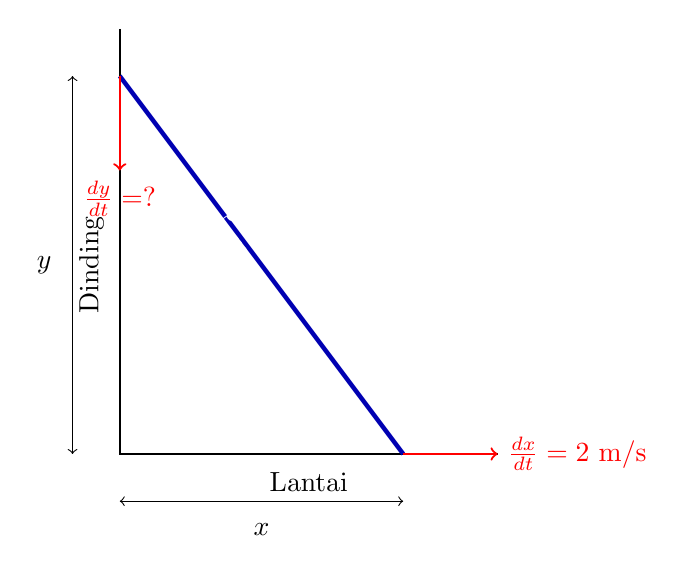
\begin{tikzpicture}[scale=1.2]
        % Dinding dan lantai
        \draw[thick] (0,4.5) -- (0,0) -- (4,0);
        \node at (-0.3, 2) [rotate=90] {Dinding};
        \node at (2, -0.3) {Lantai};

        % Tangga
        \draw[ultra thick, blue!70!black] (0,4) -- (3,0);
        \node at (1.2, 2.3) [rotate=-53, white] {5 m};

        % Jarak x dan y
        \draw[<->] (0,-0.5) -- (3,-0.5);
        \node at (1.5, -0.8) {$x$};

        \draw[<->] (-0.5,0) -- (-0.5,4);
        \node at (-0.8, 2) {$y$};

        % Vektor laju
        \draw[->, red, thick] (3,0) -- (4,0) node[right] {$\frac{dx}{dt} = 2$ m/s};
        \visible<2->{\draw[->, red, thick] (0,4) -- (0,3) node[below] {$\frac{dy}{dt} = ?$};}
      \end{tikzpicture}
    \end{column}
  \end{columns}
\end{frame}

\section{Interval Naik, Turun, dan Kecekungan Fungsi}
\begin{frame}
  \frametitle{\insertsection}
  \begin{teorema}{Uji Turunan Pertama untuk Kemonotonan}
    Misalkan $f$ kontinu pada interval $[a,b]$ dan terdiferensial pada $(a,b)$.
    \begin{itemize}
      \item Jika $f'(x) > 0$ untuk semua $x \in (a,b)$, maka $f$ \textbf{naik} pada $[a,b]$.
      \item Jika $f'(x) < 0$ untuk semua $x \in (a,b)$, maka $f$ \textbf{turun} pada $[a,b]$.
    \end{itemize}
  \end{teorema}
  \pause
  \begin{teorema}{Uji Turunan Kedua untuk Kecekungan}
    Misalkan $f$ terdiferensial dua kali pada interval terbuka $I$.
    \begin{itemize}
      \item Jika $f''(x) > 0$ untuk semua $x \in I$, maka grafik $f$ \textbf{cekung ke atas} pada $I$.
      \item Jika $f''(x) < 0$ untuk semua $x \in I$, maka grafik $f$ \textbf{cekung ke bawah} pada $I$.
    \end{itemize}
  \end{teorema}
  \pause
  \begin{definisi}{Titik Belok (Inflection Point)}
    Misalkan $f$ kontinu pada suatu interval yang memuat $c$. Titik $(c, f(c))$ disebut \textbf{titik belok} jika $f$ mengalami perubahan kecekungan di $c$ (dari cekung ke atas menjadi ke bawah, atau sebaliknya).
  \end{definisi}
\end{frame}

\begin{frame}
  \frametitle{Ilustrasi Kemonotonan dan Kecekungan}
  \centering
  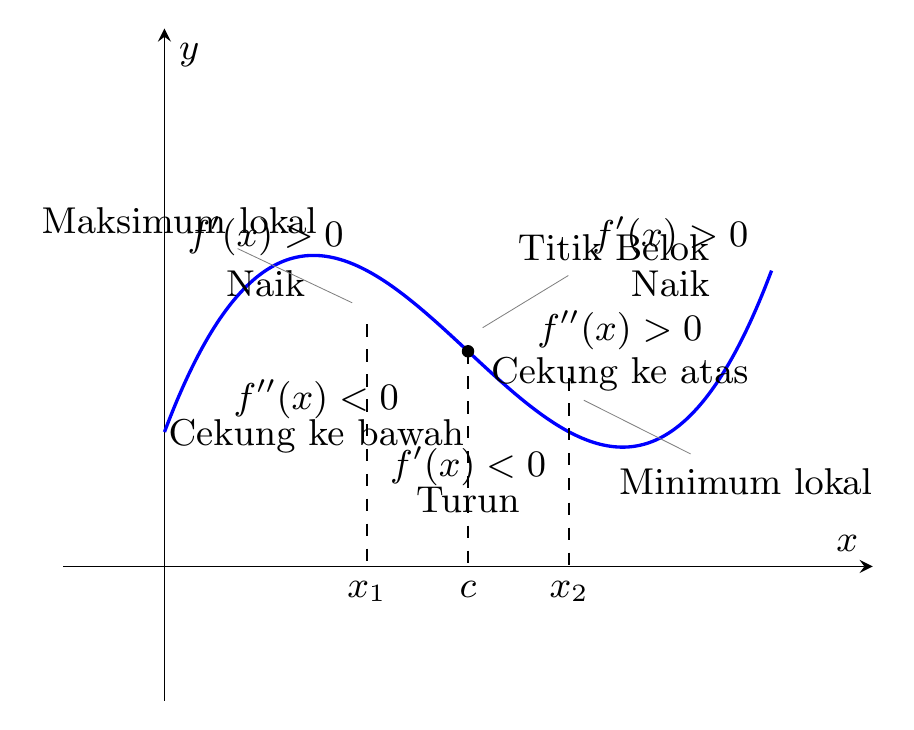
\begin{tikzpicture}[scale=1.5, every node/.style={font=\small}]
    \begin{axis}[
        axis lines=middle,
        xlabel=$x$,
        ylabel=$y$,
        xtick=\empty,
        ytick=\empty,
        xmin=-1, xmax=7,
        ymin=-1, ymax=4,
        clip=false
      ]
      \addplot[
        domain=0:6,
        samples=100,
        smooth,
        thick,
        blue,
      ] {0.1*x^3 - 0.9*x^2 + 2*x + 1};

      % Annotations
      \node[above] at (axis cs:1,2.2) {$f'(x)>0$};
      \node[above] at (axis cs:1,1.9) {Naik};

      \node[below] at (axis cs:3,1) {$f'(x)<0$};
      \node[below] at (axis cs:3,0.7) {Turun};

      \node[above] at (axis cs:5,2.2) {$f'(x)>0$};
      \node[above] at (axis cs:5,1.9) {Naik};

      \node[below] at (axis cs:1.5, 1.5) {$f''(x)<0$};
      \node[below] at (axis cs:1.5, 1.2) {Cekung ke bawah};

      \node[above] at (axis cs:4.5, 1.5) {$f''(x)>0$};
      \node[above] at (axis cs:4.5, 1.2) {Cekung ke atas};

      \draw[dashed] (axis cs:2,1.8) -- (axis cs:2,0);
      \node[below] at (axis cs:2,0) {$x_1$};
      \node[above, pin=120:Maksimum lokal] at (axis cs:2,1.8) {};

      \draw[dashed] (axis cs:4,1.4) -- (axis cs:4,0);
      \node[below] at (axis cs:4,0) {$x_2$};
      \node[below, pin=-60:Minimum lokal] at (axis cs:4,1.4) {};

      \draw[dashed] (axis cs:3,1.6) -- (axis cs:3,0);
      \node[below] at (axis cs:3,0) {$c$};
      \node[above, pin=60:Titik Belok] at (axis cs:3,1.6) {};
      \fill (axis cs:3,1.6) circle (1.5pt);

    \end{axis}
  \end{tikzpicture}
\end{frame}

\section{Ekstrim Relatif, Uji Turunan Pertama dan Kedua}
\begin{frame}
  \frametitle{\insertsection}
  \begin{definisi}{Titik Kritis}
    Misalkan $f$ terdefinisi pada interval $I$ yang memuat titik $c$. Titik $c$ disebut \textbf{titik kritis} dari $f$ jika:
    \begin{enumerate}
      \item $f'(c) = 0$ (titik stasioner), atau
      \item $f'(c)$ tidak ada (titik singular).
    \end{enumerate}
    Jika $f$ memiliki ekstrim lokal (relatif) di $c$, maka $c$ haruslah sebuah titik kritis.
  \end{definisi}
  \pause
  \begin{block}{Ekstrim Relatif (Lokal)}
    \begin{itemize}
      \item $f(c)$ adalah \textbf{maksimum relatif} jika $f(c) \ge f(x)$ untuk semua $x$ di sekitar $c$.
      \item $f(c)$ adalah \textbf{minimum relatif} jika $f(c) \le f(x)$ untuk semua $x$ di sekitar $c$.
    \end{itemize}
  \end{block}
\end{frame}

\begin{frame}
  \frametitle{Uji Ekstrim Relatif}
  \begin{alertblock}{Uji Turunan Pertama}
    Misalkan $c$ adalah titik kritis dari $f$.
    \begin{itemize}
      \item Jika tanda $f'$ berubah dari $(+)$ menjadi $(-)$ di $c$, maka $f(c)$ adalah \textbf{maksimum relatif}.
      \item Jika tanda $f'$ berubah dari $(-)$ menjadi $(+)$ di $c$, maka $f(c)$ adalah \textbf{minimum relatif}.
      \item Jika tanda $f'$ tidak berubah di $c$, maka $f(c)$ bukan ekstrim relatif.
    \end{itemize}
  \end{alertblock}
  \pause
  \begin{funfact}{Uji Turunan Kedua}
    Misalkan $f'$ dan $f''$ ada di sekitar $c$ dan $f'(c)=0$.
    \begin{itemize}
      \item Jika $f''(c) < 0$, maka $f(c)$ adalah \textbf{maksimum relatif}. (Cekung ke bawah $\implies$ puncak)
      \item Jika $f''(c) > 0$, maka $f(c)$ adalah \textbf{minimum relatif}. (Cekung ke atas $\implies$ lembah)
      \item Jika $f''(c) = 0$, uji ini gagal. Gunakan Uji Turunan Pertama.
    \end{itemize}
  \end{funfact}
\end{frame}

\section{Grafik Polinomial dan Fungsi Rasional}
\begin{frame}
  \frametitle{\insertsection}
  \begin{block}{Langkah-langkah Menggambar Grafik Fungsi $y=f(x)$}
    \begin{enumerate}
      \item \textbf{Analisis Pra-Kalkulus}:
            \begin{itemize}
              \item Tentukan domain (daerah asal) fungsi.
              \item Cari titik potong dengan sumbu-$x$ (akar) dan sumbu-$y$.
              \item Uji kesimetrian (fungsi ganjil/genap).
              \item Tentukan asimtot (tegak, datar, miring) untuk fungsi rasional.
            \end{itemize}
      \item \textbf{Analisis dengan Turunan Pertama}:
            \begin{itemize}
              \item Cari $f'(x)$. Tentukan titik kritis.
              \item Tentukan interval di mana fungsi naik ($f'(x)>0$) dan turun ($f'(x)<0$).
              \item Identifikasi ekstrim lokal menggunakan Uji Turunan Pertama.
            \end{itemize}
      \item \textbf{Analisis dengan Turunan Kedua}:
            \begin{itemize}
              \item Cari $f''(x)$.
              \item Tentukan interval di mana grafik cekung ke atas ($f''(x)>0$) dan cekung ke bawah ($f''(x)<0$).
              \item Cari titik belok.
            \end{itemize}
      \item \textbf{Sketsa Grafik}: Gabungkan semua informasi di atas untuk membuat sketsa grafik.
    \end{enumerate}
  \end{block}
\end{frame}

\section{Nilai Maksimum dan Minimum pada Suatu Fungsi}
\begin{frame}
  \frametitle{\insertsection}
  \begin{definisi}{Ekstrim Absolut (Global)}
    Misalkan $f$ terdefinisi pada interval $I$.
    \begin{itemize}
      \item $f(c)$ adalah \textbf{maksimum absolut} pada $I$ jika $f(c) \ge f(x)$ untuk semua $x \in I$.
      \item $f(c)$ adalah \textbf{minimum absolut} pada $I$ jika $f(c) \le f(x)$ untuk semua $x \in I$.
    \end{itemize}
  \end{definisi}
  \pause
  \begin{teorema}{Teorema Nilai Ekstrim}
    Jika $f$ kontinu pada interval tertutup $[a,b]$, maka $f$ pasti memiliki nilai maksimum absolut dan minimum absolut pada interval tersebut.
  \end{teorema}
  \pause
  \begin{block}{Prosedur Menemukan Ekstrim Absolut pada $[a,b]$}
    \begin{enumerate}
      \item Cari semua titik kritis $f$ pada interval terbuka $(a,b)$.
      \item Hitung nilai $f$ di setiap titik kritis yang ditemukan.
      \item Hitung nilai $f$ di titik ujung interval, yaitu $f(a)$ dan $f(b)$.
      \item Bandingkan semua nilai dari langkah 2 dan 3. Nilai terbesar adalah maksimum absolut, dan nilai terkecil adalah minimum absolut.
    \end{enumerate}
  \end{block}
\end{frame}

\begin{frame}
  \frametitle{Ilustrasi Ekstrim Absolut}
  \centering
  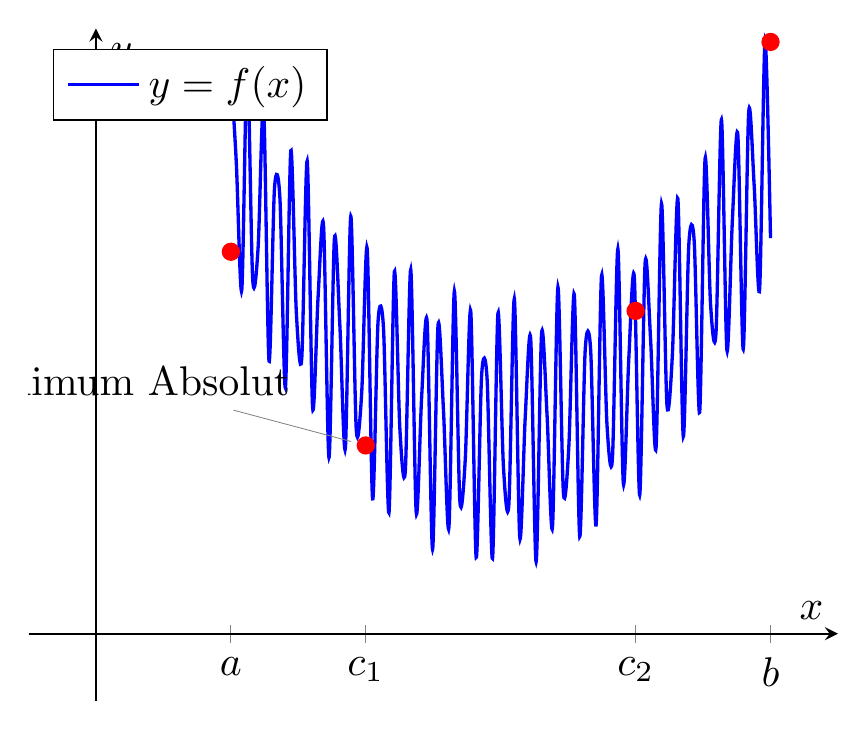
\begin{tikzpicture}[scale=1.5]
    \begin{axis}[
        axis lines=middle,
        xlabel=$x$,
        ylabel=$y$,
        xmin=-0.5, xmax=5.5,
        ymin=-0.5, ymax=4.5,
        xtick={1, 2, 4, 5},
        xticklabels={$a$, $c_1$, $c_2$, $b$},
        ytick=\empty,
        legend pos=north west
      ]
      \addplot[
        domain=1:5,
        samples=100,
        smooth,
        thick,
        blue,
      ] { (x-3)^2 * 0.5 + sin(deg(x*180/pi)) + 1.5};
      \addlegendentry{$y=f(x)$}

      % Titik-titik
      \addplot[only marks, mark=*, red, point meta=explicit symbolic] table [row sep=\\, meta=label] {
          x y label\\
          1 2.84 {Ujung interval $f(a)$}\\
          2 1.4 {Kritis (min lokal) $f(c_1)$}\\
          4 2.4 {Kritis (maks lokal) $f(c_2)$}\\
          5 4.4 {Ujung interval $f(b)$}\\
        };

      % Anotasi
      \node[pin=150:{Minimum Absolut}] at (axis cs:2, 1.4) {};
      \node[pin=90:{Maksimum Absolut}] at (axis cs:5, 4.4) {};

    \end{axis}
  \end{tikzpicture}
  \begin{itemize}
    \item Titik kritis (lokal) tidak selalu menjadi titik ekstrim absolut.
    \item Ekstrim absolut dapat terjadi di titik kritis atau di ujung interval.
  \end{itemize}
\end{frame}

\section{Aplikasi Masalah Maksimum dan Minimum}
\begin{frame}
  \frametitle{\insertsection}
  \begin{contoh}
    Sebuah kotak tanpa tutup akan dibuat dari selembar karton berbentuk persegi dengan panjang sisi 12 cm. Kotak dibuat dengan memotong empat persegi identik di setiap sudutnya, lalu melipat sisinya ke atas. Tentukan ukuran potongan agar volume kotak maksimum.
  \end{contoh}
  \pause
  \begin{columns}[T]
    \begin{column}{0.5\textwidth}
      \textbf{Solusi:}
      \begin{itemize}
        \item Misal $x$ adalah panjang sisi persegi yang dipotong. Domain $x$ adalah $(0,6)$.
        \item Dimensi kotak:
              \begin{itemize}
                \item Panjang: $p = 12 - 2x$
                \item Lebar: $l = 12 - 2x$
                \item Tinggi: $t = x$
              \end{itemize}
        \item Volume: $V(x) = (12-2x)(12-2x)x = 4x(6-x)^2 = 4(x^3 - 12x^2 + 36x)$.
        \item Cari maksimum $V(x)$. Turunkan: $V'(x) = 4(3x^2 - 24x + 36) = 12(x^2 - 8x + 12) = 12(x-2)(x-6)$.
        \item Titik kritis: $V'(x)=0 \implies x=2$ atau $x=6$.
        \item Karena domain $x \in (0,6)$, satu-satunya titik kritis yang relevan adalah $x=2$.
        \item Uji turunan kedua: $V''(x) = 12(2x-8)$. $V''(2) = 12(4-8) = -48 < 0$. Maka $x=2$ memberikan volume maksimum.
        \item Jadi, ukuran potongan adalah persegi 2 cm x 2 cm.
      \end{itemize}
    \end{column}
    \begin{column}{0.5\textwidth}
      \centering
      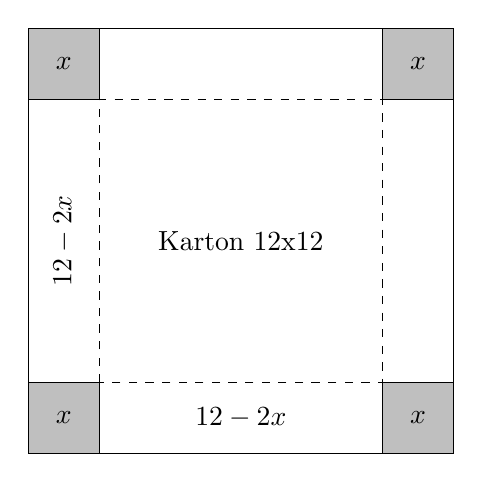
\begin{tikzpicture}[scale=0.9]
        \draw (0,0) rectangle (6,6);
        \node at (3,3) {Karton 12x12};
        \draw[dashed] (1,1) rectangle (5,5);
        \draw[fill=gray!50] (0,0) rectangle (1,1); \node at (0.5,0.5) {$x$};
        \draw[fill=gray!50] (5,0) rectangle (6,1); \node at (5.5,0.5) {$x$};
        \draw[fill=gray!50] (0,5) rectangle (1,6); \node at (0.5,5.5) {$x$};
        \draw[fill=gray!50] (5,5) rectangle (6,6); \node at (5.5,5.5) {$x$};
        \node at (3,0.5) {$12-2x$};
        \node at (0.5,3) [rotate=90] {$12-2x$};
      \end{tikzpicture}
    \end{column}
  \end{columns}
\end{frame}

\section{Teorema Rolle, Teorema Nilai Rata-rata}
\begin{frame}
  \frametitle{\insertsection}
  \begin{teorema}{Teorema Rolle}
    Misalkan $f$ adalah fungsi yang memenuhi:
    \begin{enumerate}
      \item $f$ kontinu pada interval tertutup $[a,b]$.
      \item $f$ terdiferensial pada interval terbuka $(a,b)$.
      \item $f(a) = f(b)$.
    \end{enumerate}
    Maka, ada setidaknya satu bilangan $c \in (a,b)$ sedemikian sehingga $f'(c) = 0$.
  \end{teorema}
  \pause
  \begin{block}{Interpretasi Geometris}
    Jika sebuah kurva mulus memiliki ketinggian yang sama di dua titik, maka pasti ada setidaknya satu titik di antaranya di mana garis singgungnya horizontal.
  \end{block}
  \begin{center}
    \begin{tikzpicture}[scale=1.2]
      \begin{axis}[
          axis lines=middle, xlabel=$x$, ylabel=$y$,
          xmin=-0.5, xmax=5.5, ymin=-0.5, ymax=3,
          xtick={1, 4}, xticklabels={$a$, $b$},
          ytick={1}, yticklabels={$f(a)=f(b)$}]
        \addplot[domain=1:4, smooth, thick, blue] {-(x-2.5)^2+2.5};
        \draw[dashed] (axis cs:1,1) -- (axis cs:4,1);
        \node[pin=180:{$f(a)$}] at (axis cs:1,1) {};
        \node[pin=0:{$f(b)$}] at (axis cs:4,1) {};
        % Garis singgung horizontal
        \draw[red, thick] (axis cs:2,2.75) -- (axis cs:3,2.75);
        \node[above] at (axis cs:2.5, 2.75) {$f'(c)=0$};
        \node[below] at (axis cs:2.5,0) {$c$};
        \fill (axis cs:2.5,2.75) circle (1.5pt);
      \end{axis}
    \end{tikzpicture}
  \end{center}
\end{frame}

\begin{frame}
  \frametitle{Teorema Nilai Rata-rata (TNR)}
  \begin{teorema}
    Misalkan $f$ adalah fungsi yang memenuhi:
    \begin{enumerate}
      \item $f$ kontinu pada interval tertutup $[a,b]$.
      \item $f$ terdiferensial pada interval terbuka $(a,b)$.
    \end{enumerate}
    Maka, ada setidaknya satu bilangan $c \in (a,b)$ sedemikian sehingga
    \[ f'(c) = \frac{f(b) - f(a)}{b - a} \]
  \end{teorema}
  \pause
  \begin{block}{Interpretasi Geometris}
    Pada kurva mulus antara dua titik, pasti ada setidaknya satu titik di mana garis singgungnya sejajar dengan garis sekan (tali busur) yang menghubungkan kedua titik tersebut.
  \end{block}
  \begin{center}
    \begin{tikzpicture}[scale=1.2]
      \begin{axis}[
          axis lines=middle, xlabel=$x$, ylabel=$y$,
          xmin=-0.5, xmax=5.5, ymin=-0.5, ymax=4,
          xtick={1, 5}, xticklabels={$a$, $b$},
          ytick=\empty]
        \addplot[domain=1:5, smooth, thick, blue] {0.1*(x-3)^3 + 0.5*x + 1};
        % Garis sekan
        \addplot[dashed, domain=1:5] {0.6*x + 0.5};
        \node[pin=180:{$A(a,f(a))$}] at (axis cs:1,1.1) {};
        \node[pin=0:{$B(b,f(b))$}] at (axis cs:5,3.5) {};
        % Garis singgung
        \addplot[red, thick, domain=2:4] {0.6*x + 0.23};
        \node[below] at (axis cs:3,0) {$c$};
        \fill (axis cs:3,2.03) circle (1.5pt);
      \end{axis}
    \end{tikzpicture}
  \end{center}
\end{frame}

\end{document}
